\chapter{Results and Discussion}
\section{Baseline performance of the forecasting models}
In this study, five machine leanring algorithms were trained with univariate datasets to predict the ammonia concentrations and colour levels in reclaimed water system. The forecasting model performance is presented in Fig.~\ref{fig:baseline-performance}. The performance of RF models in Fig.~\ref{fig:baseline-nh3} and Fig.~\ref{fig:baseline-colour} showed much higher test loss values compared to DNN, RNN, GRU and LSTM models. During the processes of hyperparameter turning, we discovered that the RF model performance didn't improve much when the models were trained with a varied number of estimators, while test loss values of all the other deep learning models decreased quite much toward the optimum settings of the hyperparameters.

The significant higher test loss of RF models compared to other models can be visualized by plotting the forecasted values with the ground truths (i.e., observed values). In Fig.~\ref{fig:baseline-plot}, one-step-ahead forecast horizon of ammonia concentration and colour level is plotted by RF as in Fig.~\ref{fig:baseline-nh3-plot-rf} and Fig.~\ref{fig:baseline-colour-plot-rf} and LSTM models as in Fig.~\ref{fig:baseline-nh3-plot-lstm} and Fig.~\ref{fig:baseline-colour-plot-lstm}. It's easier to observe that the RF models are less capable of predicting the water quality paratmers. 

\begin{figure}[h]
    \centering
    \begin{subfigure}[t]{0.45\textwidth}
      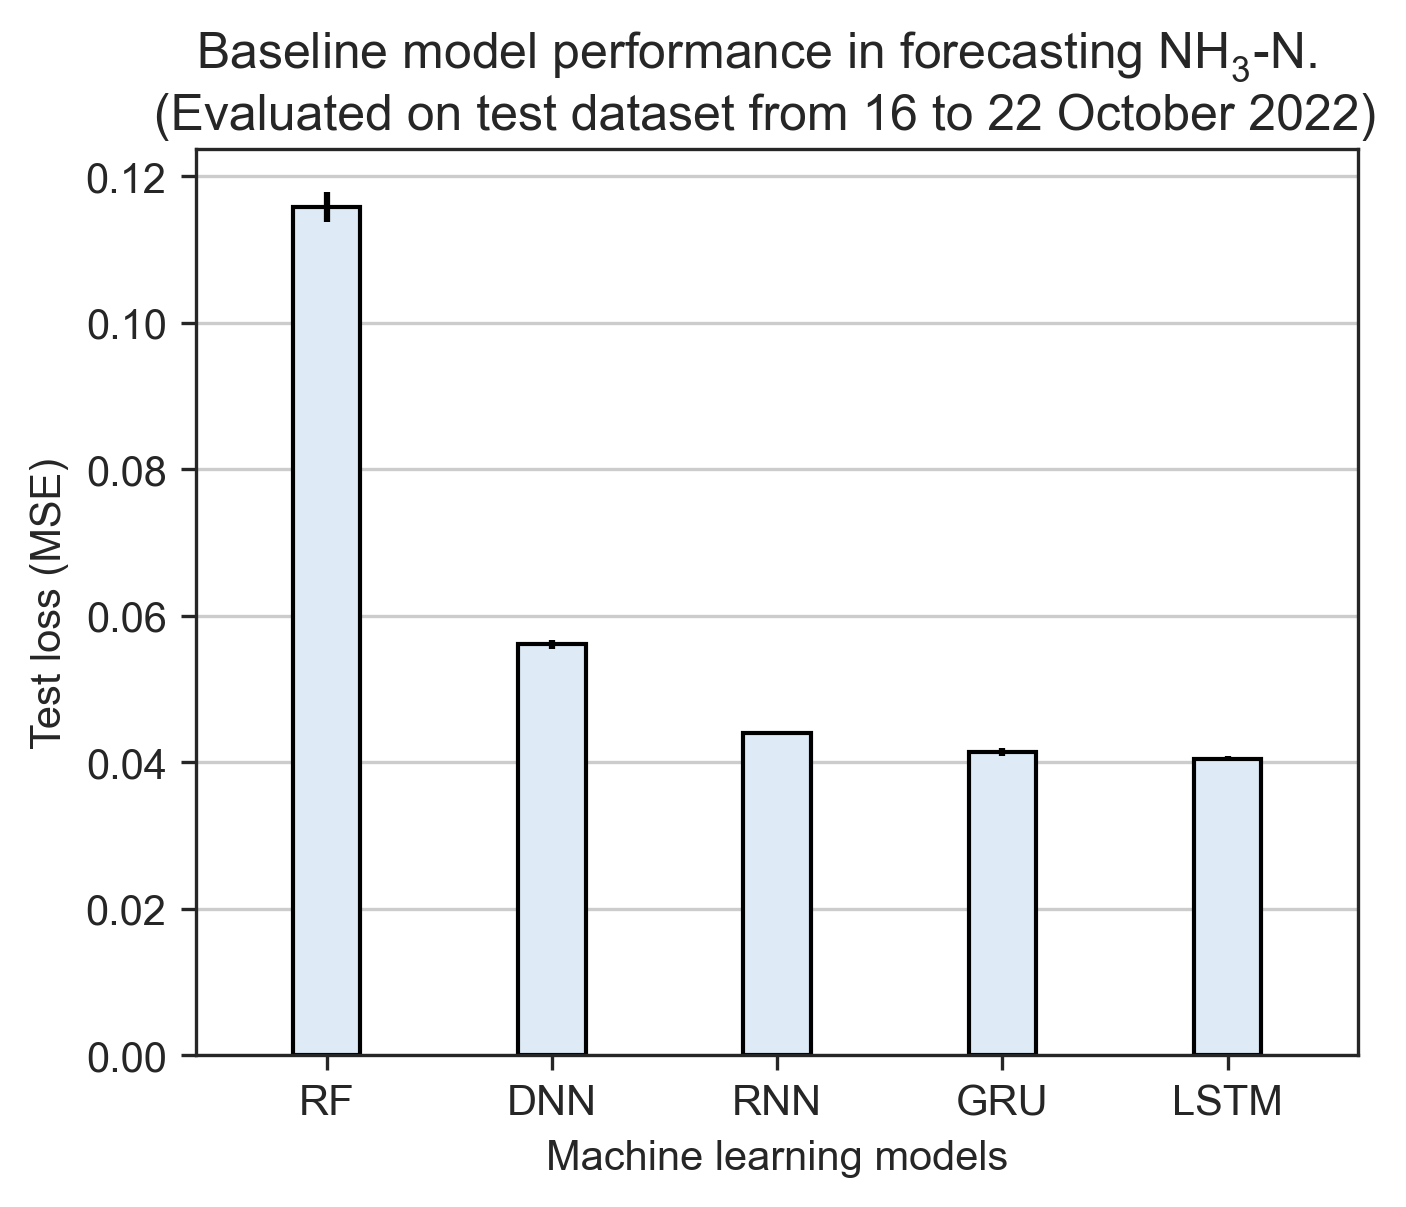
\includegraphics[width=\linewidth]{imgs/results/baseline-models-nh3.png}
      \caption{Test loss values from five ammonia forecasting models.} \label{fig:baseline-nh3}
    \end{subfigure}%
    \hspace{2em}%   % maximize separation between the subfigures
    \begin{subfigure}[t]{0.45\textwidth}
      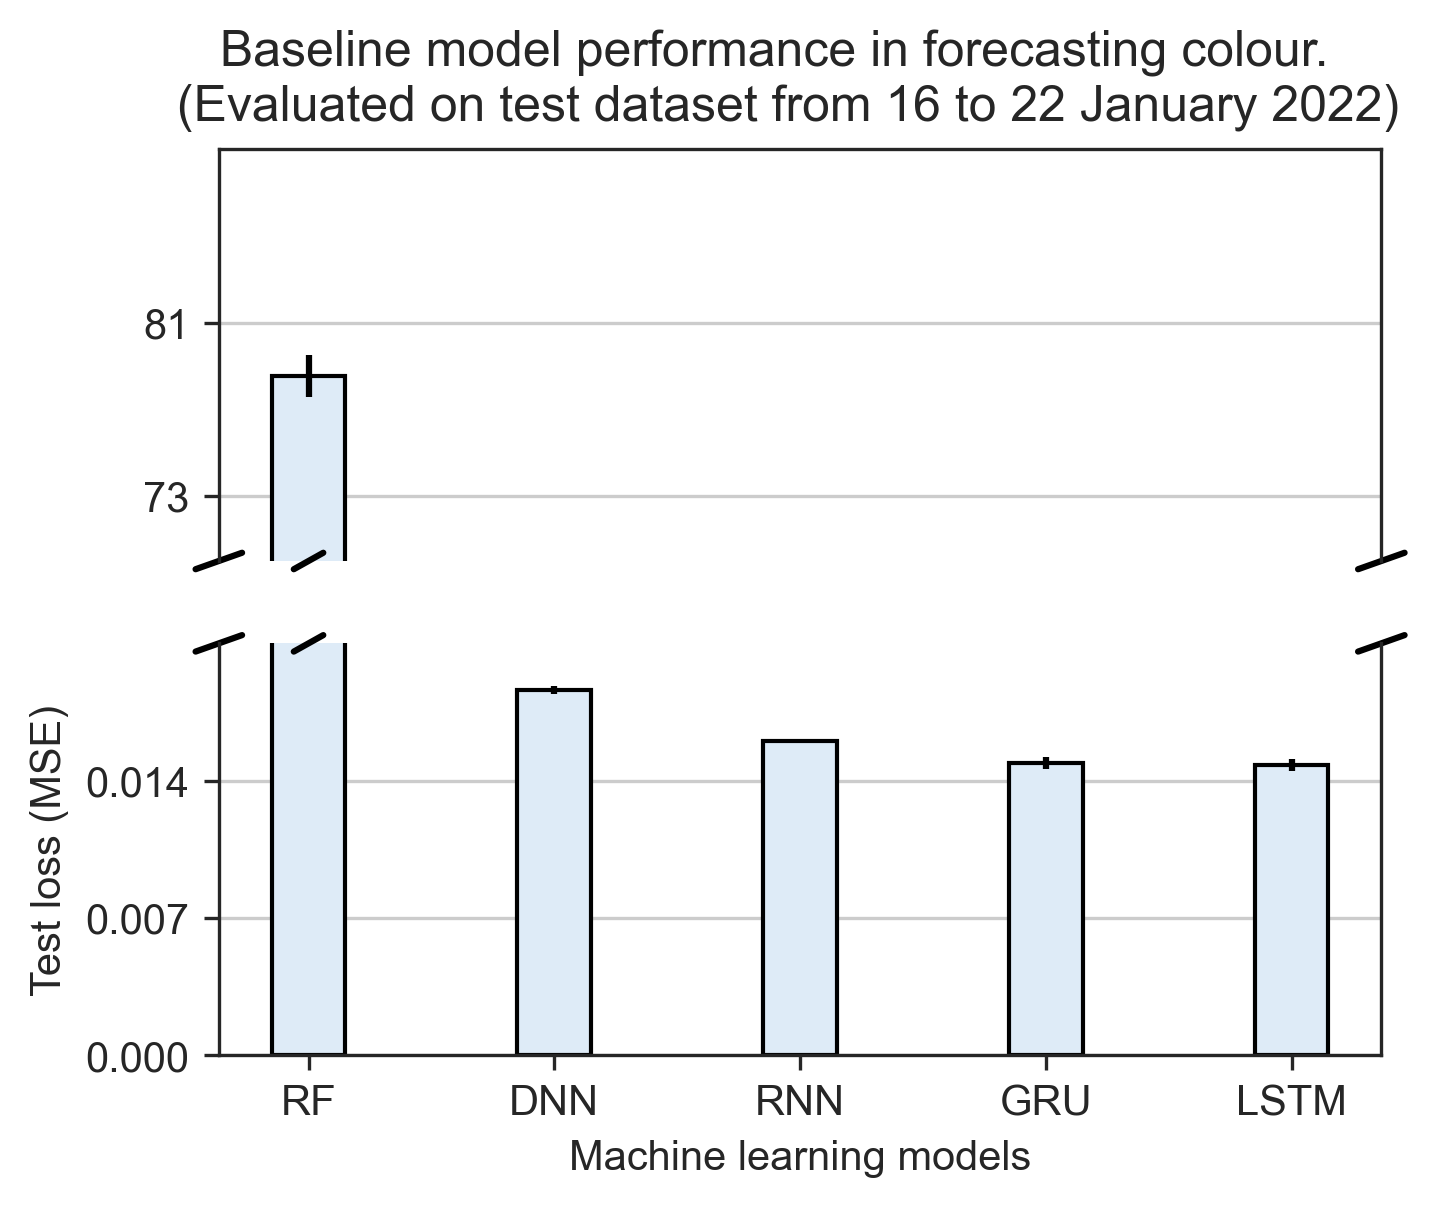
\includegraphics[width=\linewidth]{imgs/results/baseline-models-colour.png}
      \caption{Test loss values from five colour forecasting models.} \label{fig:baseline-colour}
    \end{subfigure}%  
  \caption{Baseline performance of ammonia and colour forecasting models.} \label{fig:baseline-performance}
\end{figure}

\begin{figure}[h]
    \centering
    \hspace{1em}%
    \begin{subfigure}[t]{0.45\textwidth}
      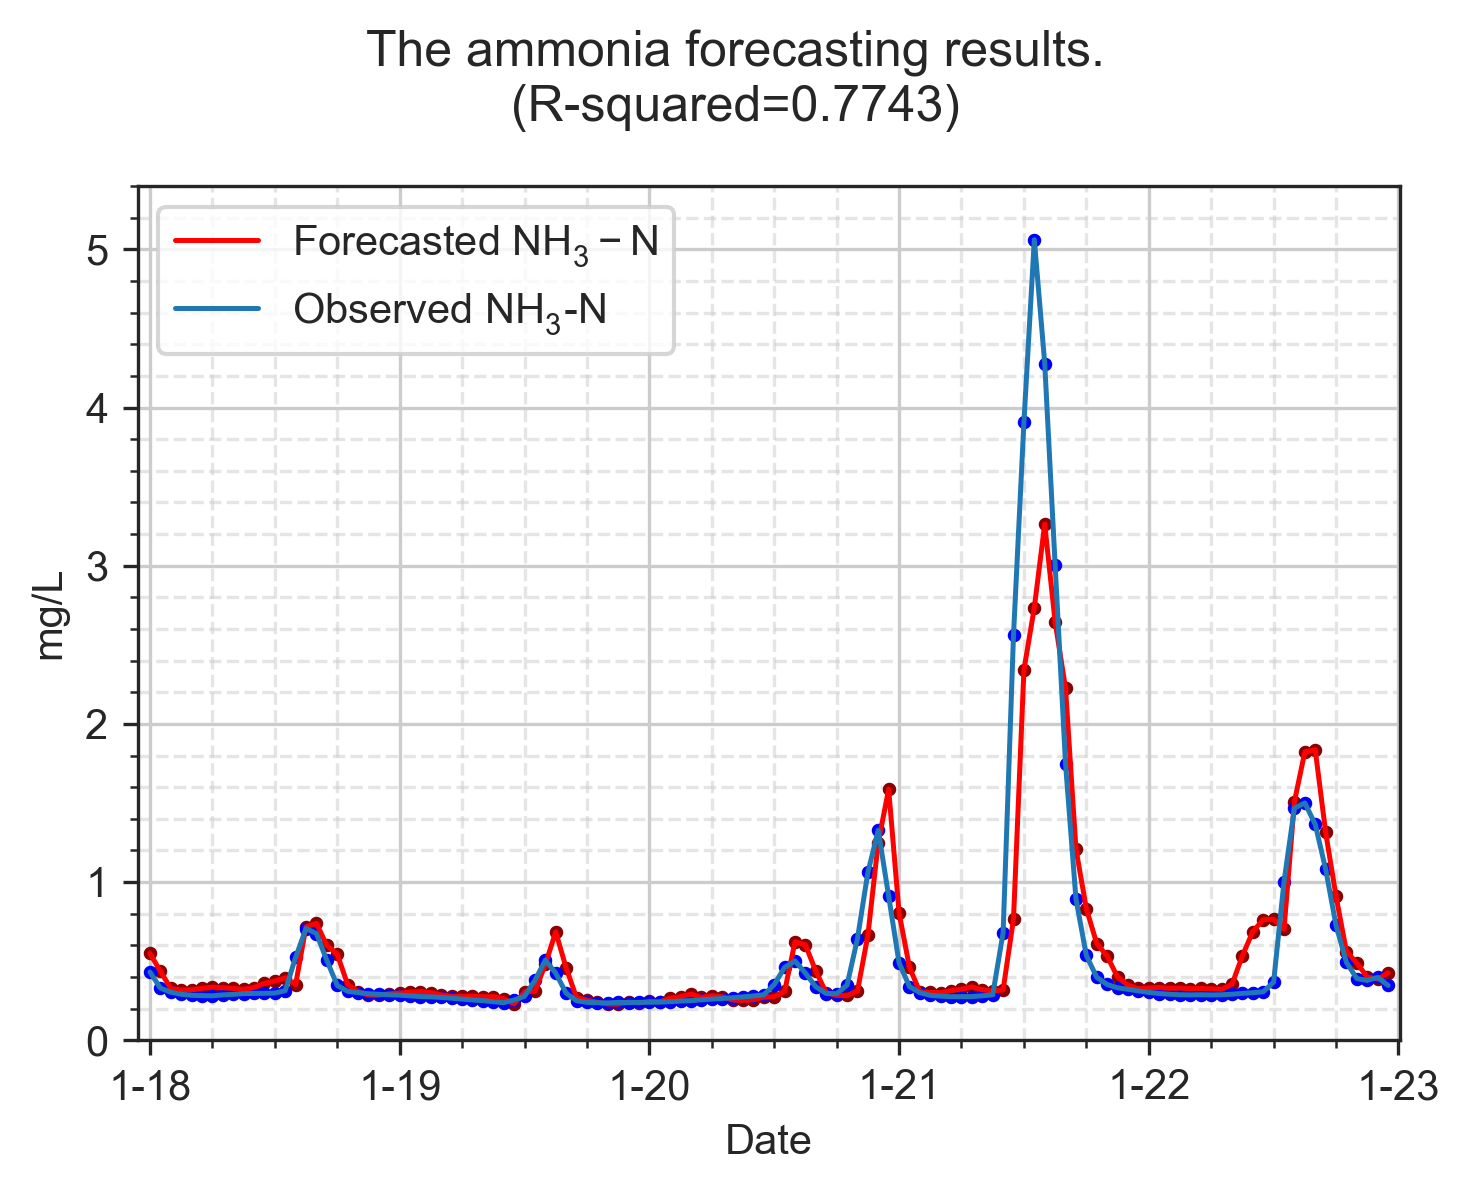
\includegraphics[width=\linewidth]{imgs/results/ammonia-colour-forecast-plot/00-RF_1_pred_Step1-obs-nh3.png}
      \caption{Baseline RF model forecasting ammonia concentration.} \label{fig:baseline-nh3-plot-rf}
    \end{subfigure}%
    \hspace{1em}%   % maximize separation between the subfigures
    \begin{subfigure}[t]{0.45\textwidth}
      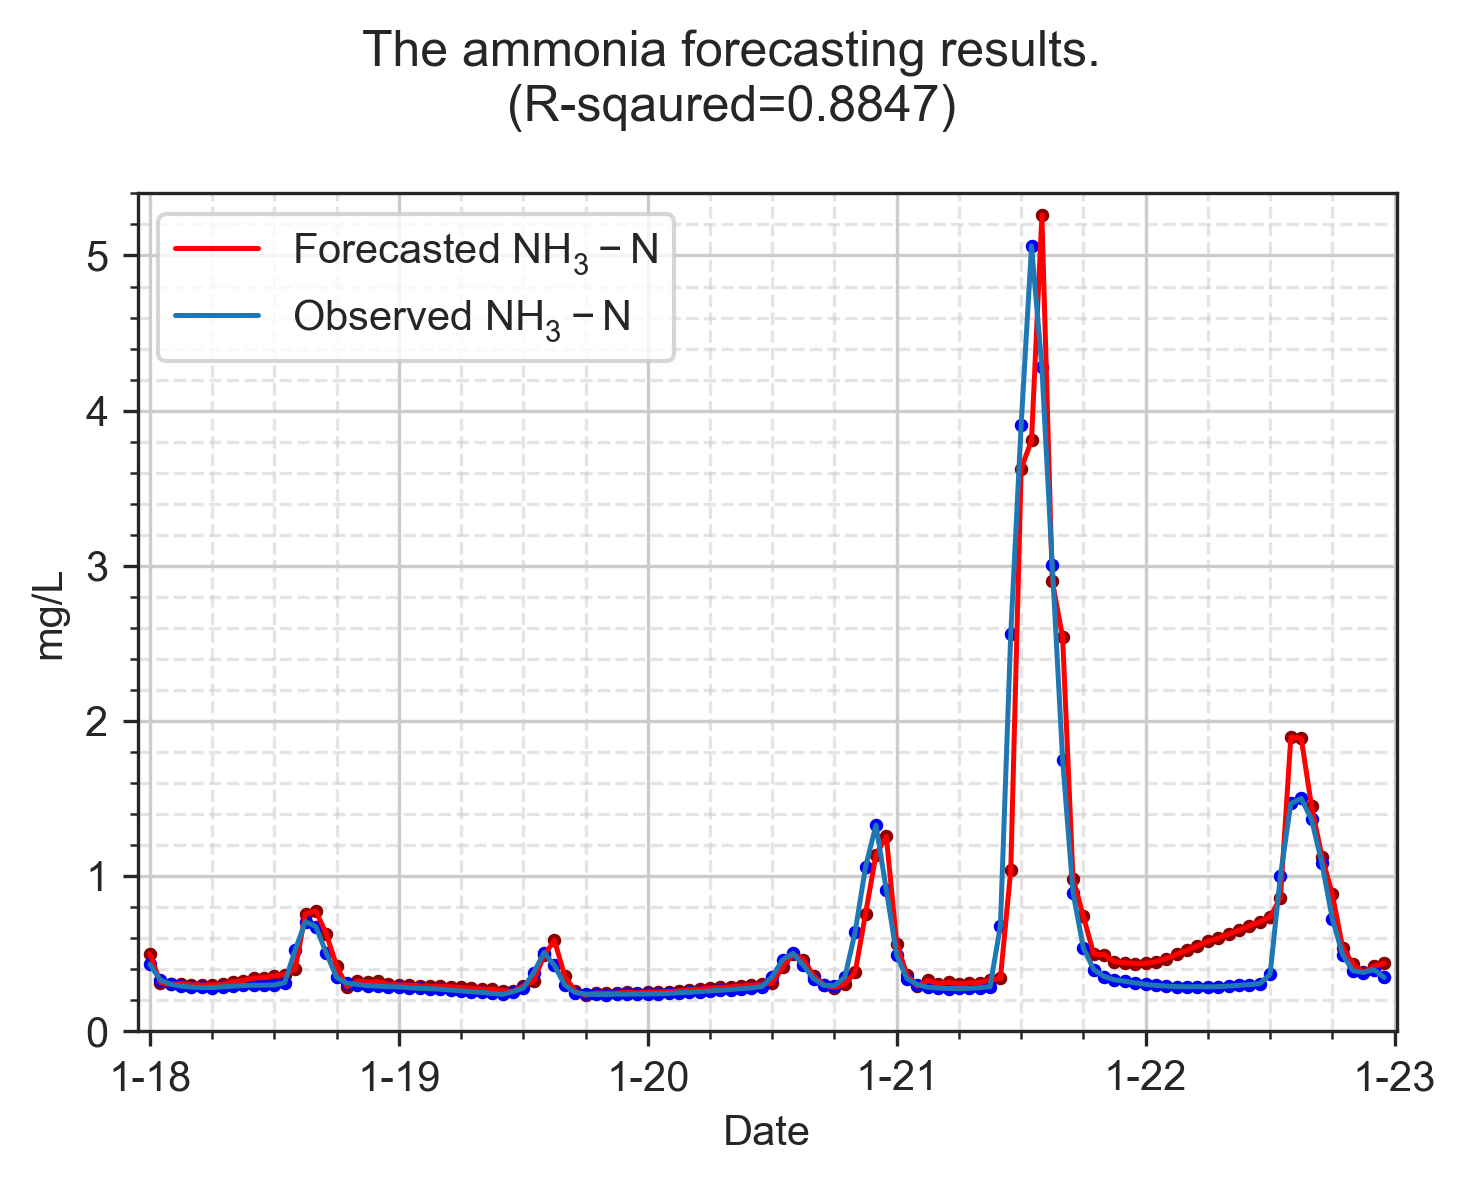
\includegraphics[width=\linewidth]{imgs/results/ammonia-colour-forecast-plot/00-LSTM_1_pred_Step1-obs-nh3.png}
      \caption{Baseline LSTM model forecasting ammonia concentration.} \label{fig:baseline-nh3-plot-lstm}
    \end{subfigure}%
    \hspace{1em}%   % maximize separation between the subfigures
    \begin{subfigure}[t]{0.45\textwidth}
      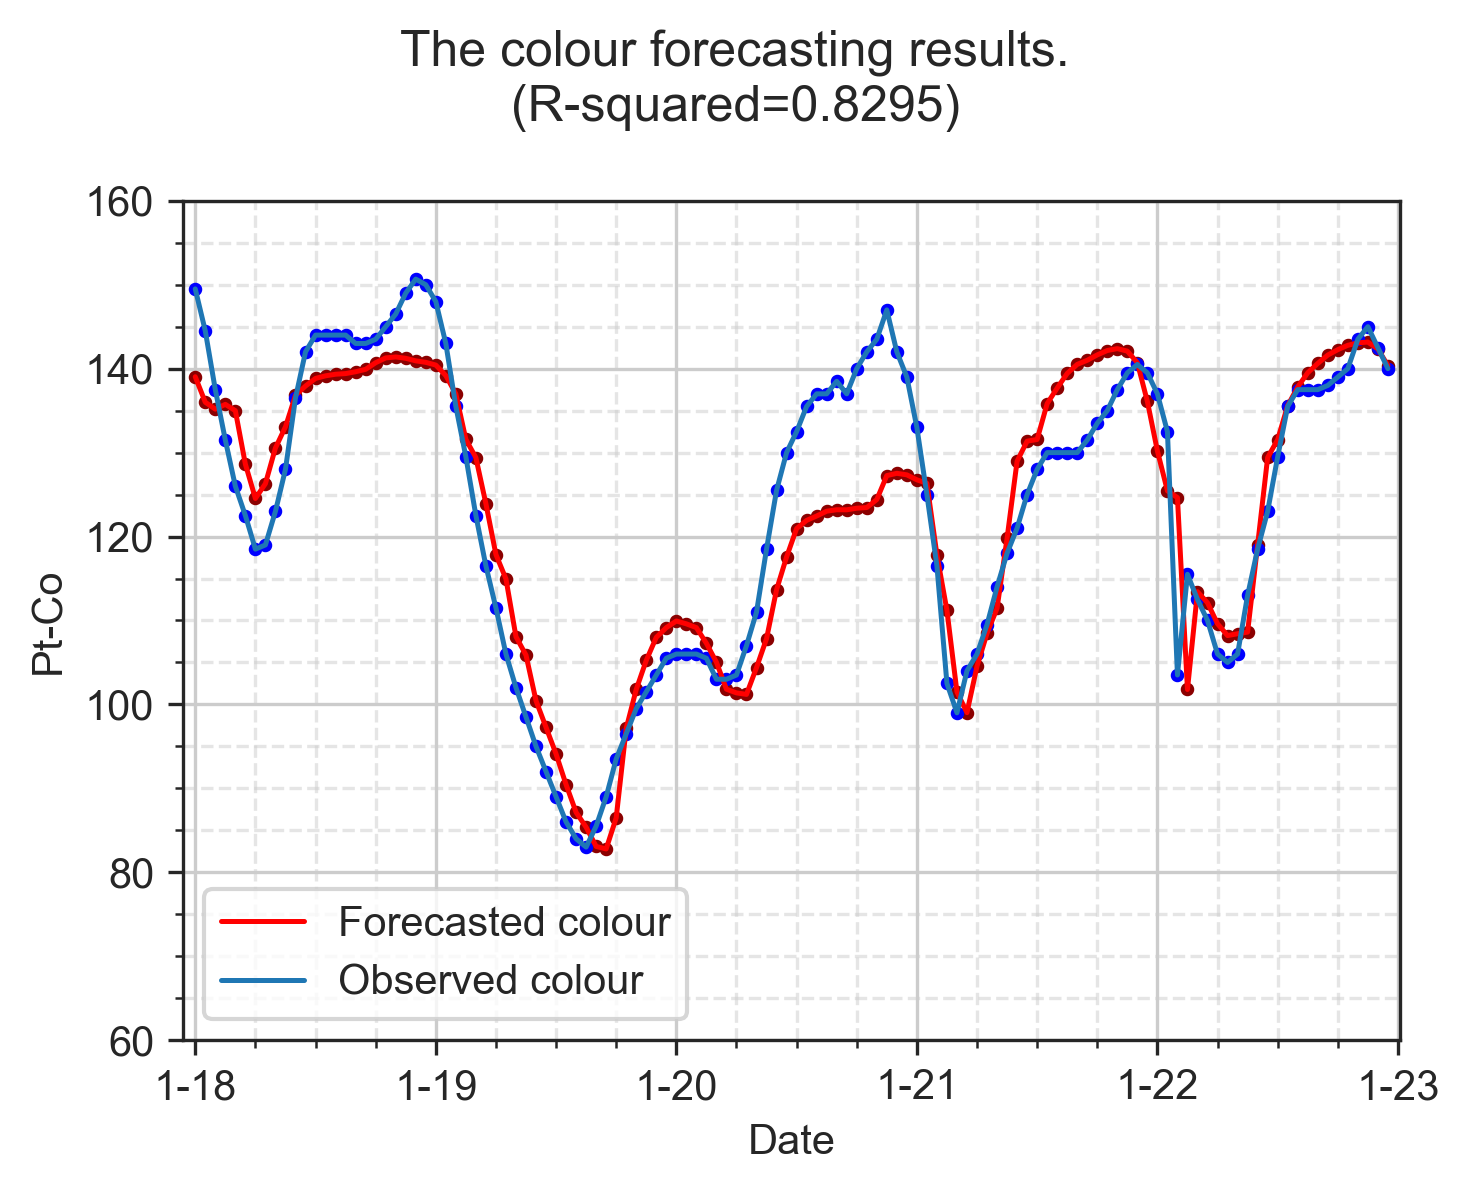
\includegraphics[width=\linewidth]{imgs/results/ammonia-colour-forecast-plot/00-RF_1_pred_Step1-obs-colour.png}
      \caption{Baseline RF model forecasting colour levels.} \label{fig:baseline-colour-plot-rf}
    \end{subfigure}% 
    \hspace{1em}%   % maximize separation between the subfigures
    \begin{subfigure}[t]{0.45\textwidth}
      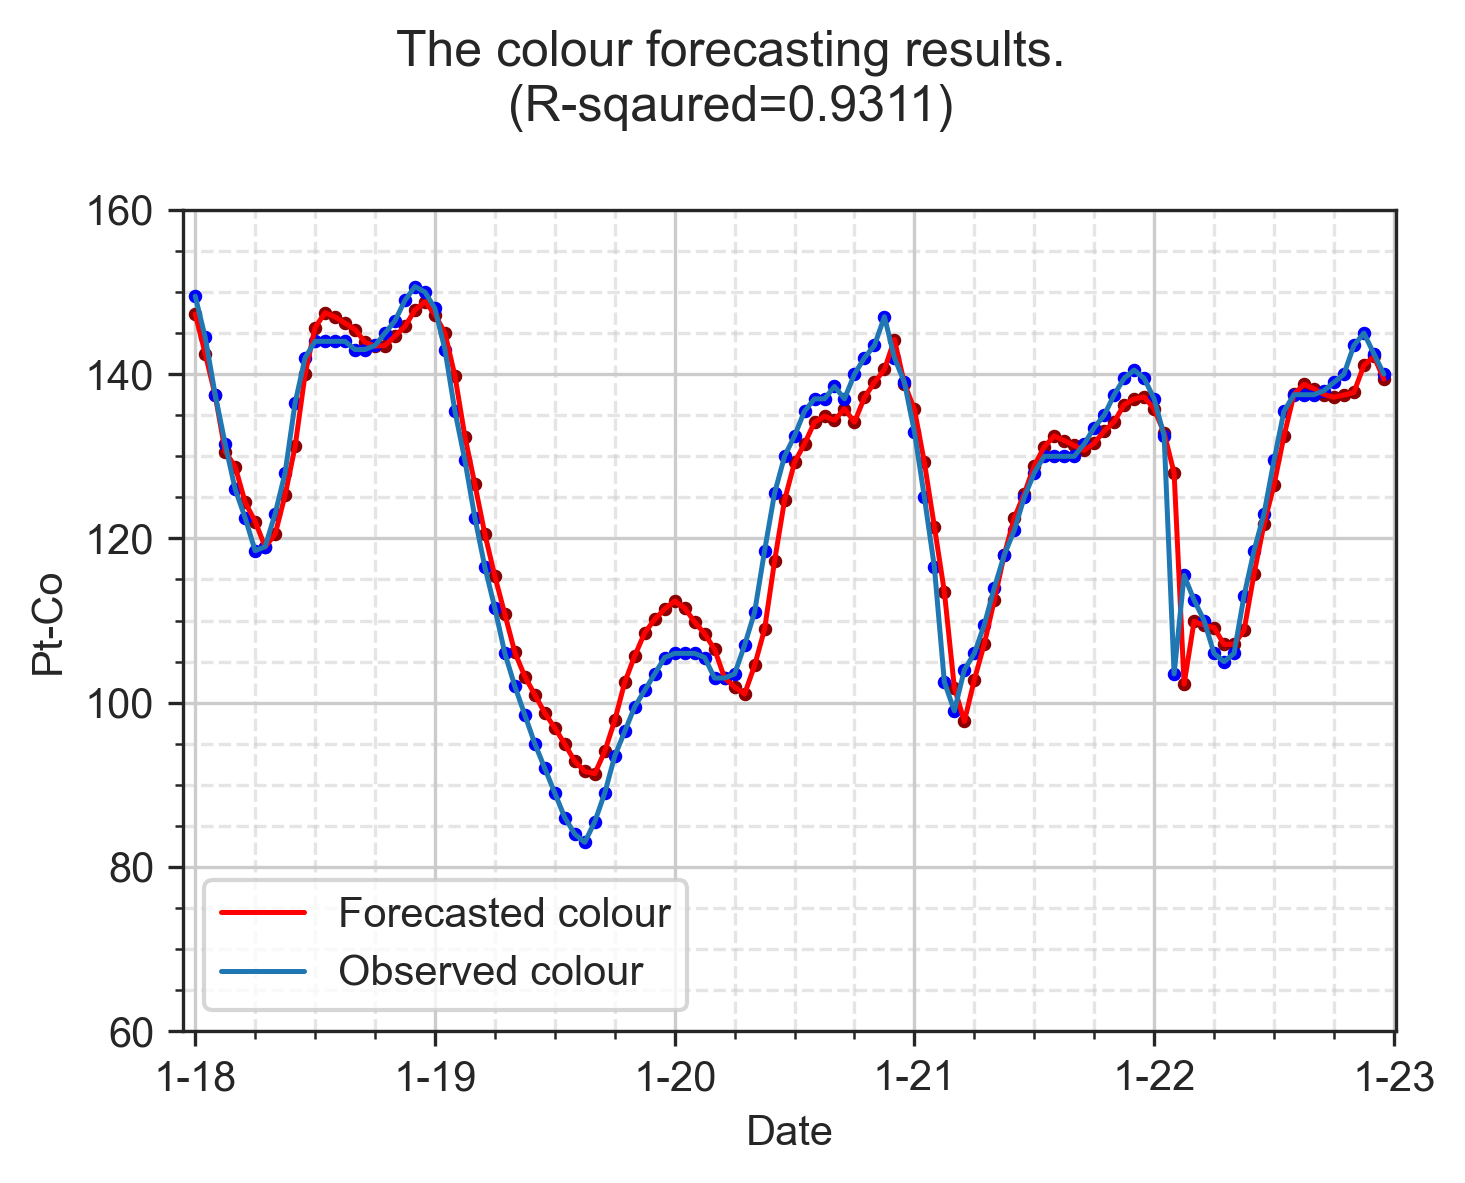
\includegraphics[width=\linewidth]{imgs/results/ammonia-colour-forecast-plot/00-LSTM_1_pred_Step1-obs-colour.png}
      \caption{Baseline LSTM model forecasting colour levels.} \label{fig:baseline-colour-plot-lstm}
    \end{subfigure}% 
  \caption{Visulization of the model forecasting results.} \label{fig:baseline-plot}
\end{figure}

\section{Improved performance on forecasting models using data pre-processing techniques}
\subsection{Models trained by pre-processed datasets}
In this study, we investigate whether the datasets treated by the proposed data pre-processing methods can improve the baseline model performance using the same hyperparameter settings. As shown in Table.~\ref{tab:baseline-result-jan-nh3} and Table.~\ref{tab:baseline-result-jan-colour}, we listed all the test loss values of five machine learning algorithms trained with each proposed pre-processed methods for ammonia concentrations and colour levels forecasting. The machine learning algorithm trained by datasets which were applied with SG filters at different window sizes are denoted as model-sg5, model-sg7, model-sg9; the naming rule applies the same to datasets applied with EWMA filters; for the method of outlier removal for ammonia data is denoted as model-or; models trained with the raw datasets are denote as model-obs (i.e., observed dataset).

\begin{table}[!ht]
  \centering
  \caption{Baseline performance of ammonia forecasting model, evaluated on test dataset from \textbf{16 to 22 Janurary 2022}. Loss values are calculated by MSE.}\label{tab:baseline-result-jan-nh3}
  \begin{NiceTabular}{lcclcc}
      \toprule
      Model-Dataset & Test loss & Valid loss & Model-Dataset & Test loss & Valid loss \\
      \midrule
      GRU-sg7  & 0.0383 &1.2508&RNN-or  & 0.0432&1.6345 \\
      GRU-sg5  & 0.0385 &1.2644&RNN-ew3 & 0.0434&1.6041 \\
      LSTM-ew3 & 0.0388 &1.0796&RNN-obs & 0.0440&1.6734 \\
      LSTM-sg5 & 0.0388 &1.2346&RNN-sg9 & 0.0442&1.7046 \\
      LSTM-sg7 & 0.0388 &1.1804&DNN-obs & 0.0561&3.2383 \\
      GRU-ew2  & 0.0389 &1.1891&DNN-sg5 & 0.0562&3.2170 \\
      GRU-ew4  & 0.0391 &1.2390&DNN-ew2 & 0.0563&3.1677 \\
      GRU-ew3  & 0.0392 &1.2199&DNN-ew3 & 0.0569&3.2317 \\
      LSTM-ew2 & 0.0392 &1.0969&DNN-sg7 & 0.0570&3.2014 \\
      LSTM-ew4 & 0.0395 &1.1219&DNN-ew4 & 0.0571&3.2188 \\
      GRU-sg9  & 0.0396 &1.3097&DNN-or  & 0.0572&3.1972 \\
      LSTM-or  & 0.0398 &1.2612&DNN-sg9 & 0.0574&3.2484 \\
      LSTM-obs & 0.0405 &1.3993&RF-obs  & 0.1158&- \\
      GRU-or   & 0.0405 &1.2366&RF-sg9  & 0.1196&- \\
      LSTM-sg9 & 0.0410 &1.3076&RF-ew2  & 0.1286&- \\
      GRU-obs  & 0.0414 &1.3638&RF-or   & 0.1294&- \\
      RNN-sg5  & 0.0415 &1.5088&RF-sg5  & 0.1298&- \\
      RNN-ew2  & 0.0421 &1.5425&RF-ew3  & 0.1313&- \\
      RNN-sg7  & 0.0423 &1.6267&RF-sg7  & 0.1409&- \\
      RNN-ew4  & 0.0432 &1.5992&RF-ew4  & 0.1441&- \\
      \bottomrule
  \end{NiceTabular}
\end{table}

The improvements on the performance of ammonia forecasting models are most significant with the use of SG filters. GRU-sg5 and GRU-sg7 reduced 7.0\% and 7.4\% in the test loss compared with GRU-obs, while LSTM-sg5 and LSTM-sg7 reduced 4.2\% of the test loss compared to LSTM-obs. Both data smoothing filters reduced the test loss and the improvements can be attributed to the modified relationships bewteen each datapoints. The SG filters modified the original datapoints by covoluting with both previous and the following datapoints, which resembles the working mechanisms of recurrent neural networks, while the EWMA filter modified the datapoints by averaging the value of current datapoint with previous ones. The performance of RF models was the poorest in the baseline model performance compared to other models. The results presented in Table.~\ref{tab:baseline-result-jan-nh3} indicate despite RF models were trained with data pre-processing methods, the model performance in test loss was still much higher than the poorest deep learning model, which is DNN-sg9 in this case.

Empirically, when different models are evaluated by the same testing dataset, the best Model-Dataset combination shold have both the lowest values of test and validation loss. For instance, GRU-sg7 model in forecasting ammonia has the lowest test loss of 0.0383, yet the validation loss of 1.2508 only ranks the tenth from the smallest validation loss vlaues. The models with top three lowest values of the validation loss are LSTM-ew3, LSTM-ew2 and LSTM-ew4. This finding points to the potential of the heterogeneity between the trianing and testing datasets. This hypothesis was the explanation with the highest likelihood when no overfitting was observed in the training datasets. Further tests were carried out using testing dataset from October to examine how the Model-Dataset ranks of test and validation loss values will change into. To the best of my understanding, the comparisons between testing and validation loss are not discussed on the currently available research papers in modelling of wastewater treatment industry.

As shown in Table.~\ref{tab:baseline-result-oct-nh3}, the top three ranks of Model-Dataset in the lowest validation loss is the same to the top three ranks in the test loss values. This is in good agreement with how the heterogeneity of the datasets can impact on the model performance. The evluations of the ammonia forecasting models in October 2021 showed a complete different outcomes compared to the one in January 2022. Surpirsingly, the top three ranks of Model-Dataset in the lowest validation loss are the same of the lowest test loss, which are 0.0158 from LSTM-ew3, 0.0161 from LSTM-ew2, and 0.0163 from LSTM-ew4. Instead of GRU, LSTM becomes the best model for training ammonia forecasting model. The most remarkable results in Table.~\ref{tab:baseline-result-oct-nh3} is that EWMA filter seems to be the most ideal pre-processing methods for traning deep learning models as LSTM-ew3, GRU-ew3, RNN-ew4 and DNN-ew3 models showed the best model performance in test loss compared to the same models trained by other data pre-processing methods.

\begin{table}[!ht]
    \centering
    \caption{Baseline performance of ammonia forecasting model, evaluated on test dataset from \textbf{10 to 16 October 2021}. Loss values are calculated by MSE.}\label{tab:baseline-result-oct-nh3}
    \begin{NiceTabular}{lcclcc}
        \toprule
        Model-Dataset & Test loss & Valid loss & Model-Dataset & Test loss & Valid loss \\
        \midrule
        LSTM-ew3 & 0.0158 & 1.0796 & RNN-or  & 0.0197 & 1.6345 \\
        LSTM-ew2 & 0.0161 & 1.0969 & RNN-sg7 & 0.0201 & 1.6267 \\
        LSTM-ew4 & 0.0163 & 1.1219 & RNN-sg9 & 0.0205 & 1.7046 \\
        LSTM-sg5 & 0.0166 & 1.2346 & RNN-obs & 0.0206 & 1.6734 \\
        GRU-ew3  & 0.0167 & 1.2199 & DNN-ew3 & 0.0316 & 3.2317 \\
        GRU-ew4  & 0.0169 & 1.2390 & DNN-or  & 0.0316 & 3.1972 \\
        GRU-ew2  & 0.0170 & 1.1891 & DNN-sg7 & 0.0316 & 3.2014 \\
        GRU-sg9  & 0.0174 & 1.3097 & DNN-ew2 & 0.0318 & 3.1677 \\
        LSTM-obs & 0.0175 & 1.2366 & DNN-ew4 & 0.0319 & 3.2188 \\
        LSTM-or  & 0.0177 & 1.2612 & DNN-obs & 0.0319 & 3.2383 \\
        GRU-sg5  & 0.0178 & 1.2644 & DNN-sg5 & 0.0319 & 3.2170 \\
        GRU-sg7  & 0.0180 & 1.2508 & DNN-sg9 & 0.0319 & 3.2484 \\
        LSTM-sg7 & 0.0180 & 1.1804 & RF-sg9  & 0.1307 & - \\
        GRU-or   & 0.0187 & 1.3993 & RF-sg7  & 0.1311 & - \\
        LSTM-sg9 & 0.0188 & 1.3076 & RF-sg5  & 0.1343 & - \\
        GRU-obs  & 0.0189 & 1.3638 & RF-ew2  & 0.1346 & - \\
        RNN-ew4  & 0.0190 & 1.5992 & RF-ew3  & 0.1368 & - \\
        RNN-ew2  & 0.0191 & 1.5425 & RF-obs  & 0.1443 & - \\
        RNN-ew3  & 0.0193 & 1.6041 & RF-ew4  & 0.1451 & - \\
        RNN-sg5  & 0.0195 & 1.5088 & RF-or   & 0.1477 & - \\
        \bottomrule
    \end{NiceTabular}
\end{table}

The test loss values of the colour forecasting models are presented in Table.~\ref{tab:baseline-result-jan-colour}. The best performed colour forecasting models are the LSTM models trained by EWMA filters, which are 0.0136 from LSTM-ew4, 0.0138 from LSTM-ew2 and LSTM-ew3. Interestingly, LSTM models trained by EWMA also showed the best performance in ammonia forecasting models. The top three ranks of Model-Dataset in the lowest validation loss ranks the 6th, 20th, and 1st from the lowest test loss values. However, we don't have extra testing datasets for re-evaluating the colour forecasting models. Compromises have to be made during the analysis of colour forecasting models.

\begin{table}[!ht]
  \centering
  \caption{Baseline performance of colour forecasting model, evaluated on test dataset from \textbf{16 to 22 Janurary 2022}. Loss values are calculated by MSE.}\label{tab:baseline-result-jan-colour}
  \begin{NiceTabular}{lcclcc}
      \toprule
      Model-Dataset & Test loss & Valid loss & Model-Dataset & Test loss & Valid loss \\
      \midrule
      LSTM-ew4 & 0.0136 &0.7515&RNN-obs  & 0.0160 &1.0623 \\
      LSTM-ew2 & 0.0138 &0.8011&LSTM-sg7 & 0.0161 &0.7439 \\
      LSTM-ew3 & 0.0138 &0.7547&LSTM-sg5 & 0.0168 &0.8355 \\
      GRU-ew3  & 0.0140 &0.8068&DNN-sg5  & 0.0180 &1.4702 \\
      GRU-ew2  & 0.0142 &0.8330&DNN-sg7  & 0.0180 &1.4823 \\
      GRU-ew4  & 0.0143 &0.7694&DNN-sg9  & 0.0180 &1.4574 \\
      LSTM-sg9 & 0.0143 &0.7137&DNN-ew4  & 0.0181 &1.4632 \\
      RNN-ew3  & 0.0144 &0.8492&DNN-ew3  & 0.0182 &1.4716 \\
      RNN-ew4  & 0.0147 &0.8476&DNN-ew2  & 0.0183 &1.4946 \\
      RNN-sg9  & 0.0147 &0.8363&DNN-obs  & 0.0186 &1.5397 \\
      LSTM-obs & 0.0148 &0.9744&RF-sg9   & 63.6847& \\
      GRU-obs  & 0.0149 &0.9927&RF-sg7   & 73.8263& \\
      RNN-ew2  & 0.0150 &0.9083&RF-ew3   & 75.1974&- \\
      GRU-sg9  & 0.0151 &0.7575&RF-ew4   & 77.8829&- \\
      RNN-sg5  & 0.0158 &0.8846&RF-obs   & 78.5296&- \\
      RNN-sg7  & 0.0158 &0.8755&RF-ew2   & 78.8753&- \\
      GRU-sg7  & 0.0159 &0.7791&RF-sg5   & 81.0696&- \\
      GRU-sg5  & 0.0160 &0.8080&    -    &     -  &- \\
      \bottomrule
  \end{NiceTabular}
\end{table}

By comparing the baseline performance and the influences of data pre-processing methods on machine learning models, our findings appear to be well substantiated the use of LSTM models for training ammonia and colour forecasting models due to it's outstanding model performance evaluated by test loss values. Although EWMA filters showed surprising effects on improving the performance of most models, the influence of pre-processing methods are still not consistant across different models and training datasets. Thus, in the testings of the proposed model training processes will include all the pre-processing methods for model training, and LSTM will be used as the only machine learning model.

\subsection{The effect of window size of data smoothing filters}

\begin{figure}[h]
  \centering
  \begin{subfigure}[t]{0.45\textwidth}
    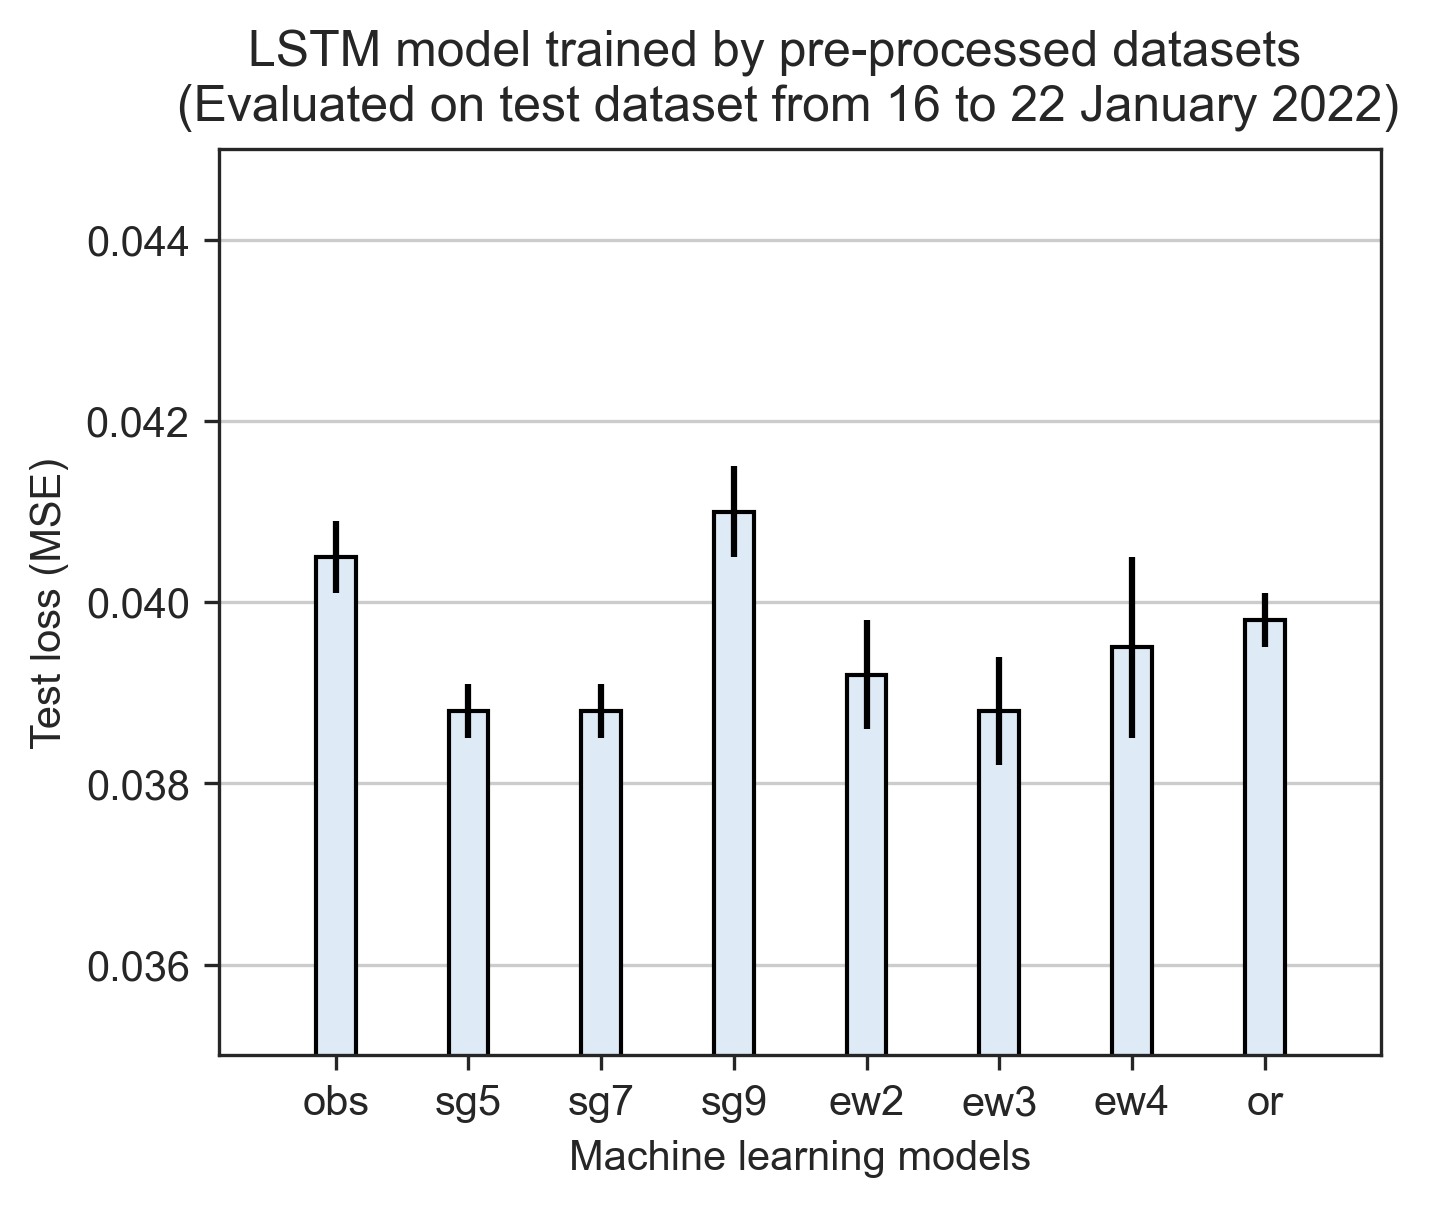
\includegraphics[width=\linewidth]{imgs/results/feature-engineering/pre-processing-nh3-jan.png}
    \caption{Baseline performance of ammonia forecasting models trained by LSTM.} \label{fig:preprocessing-nh3}
  \end{subfigure}
  \hspace{2em}
  \begin{subfigure}[t]{0.45\textwidth}
    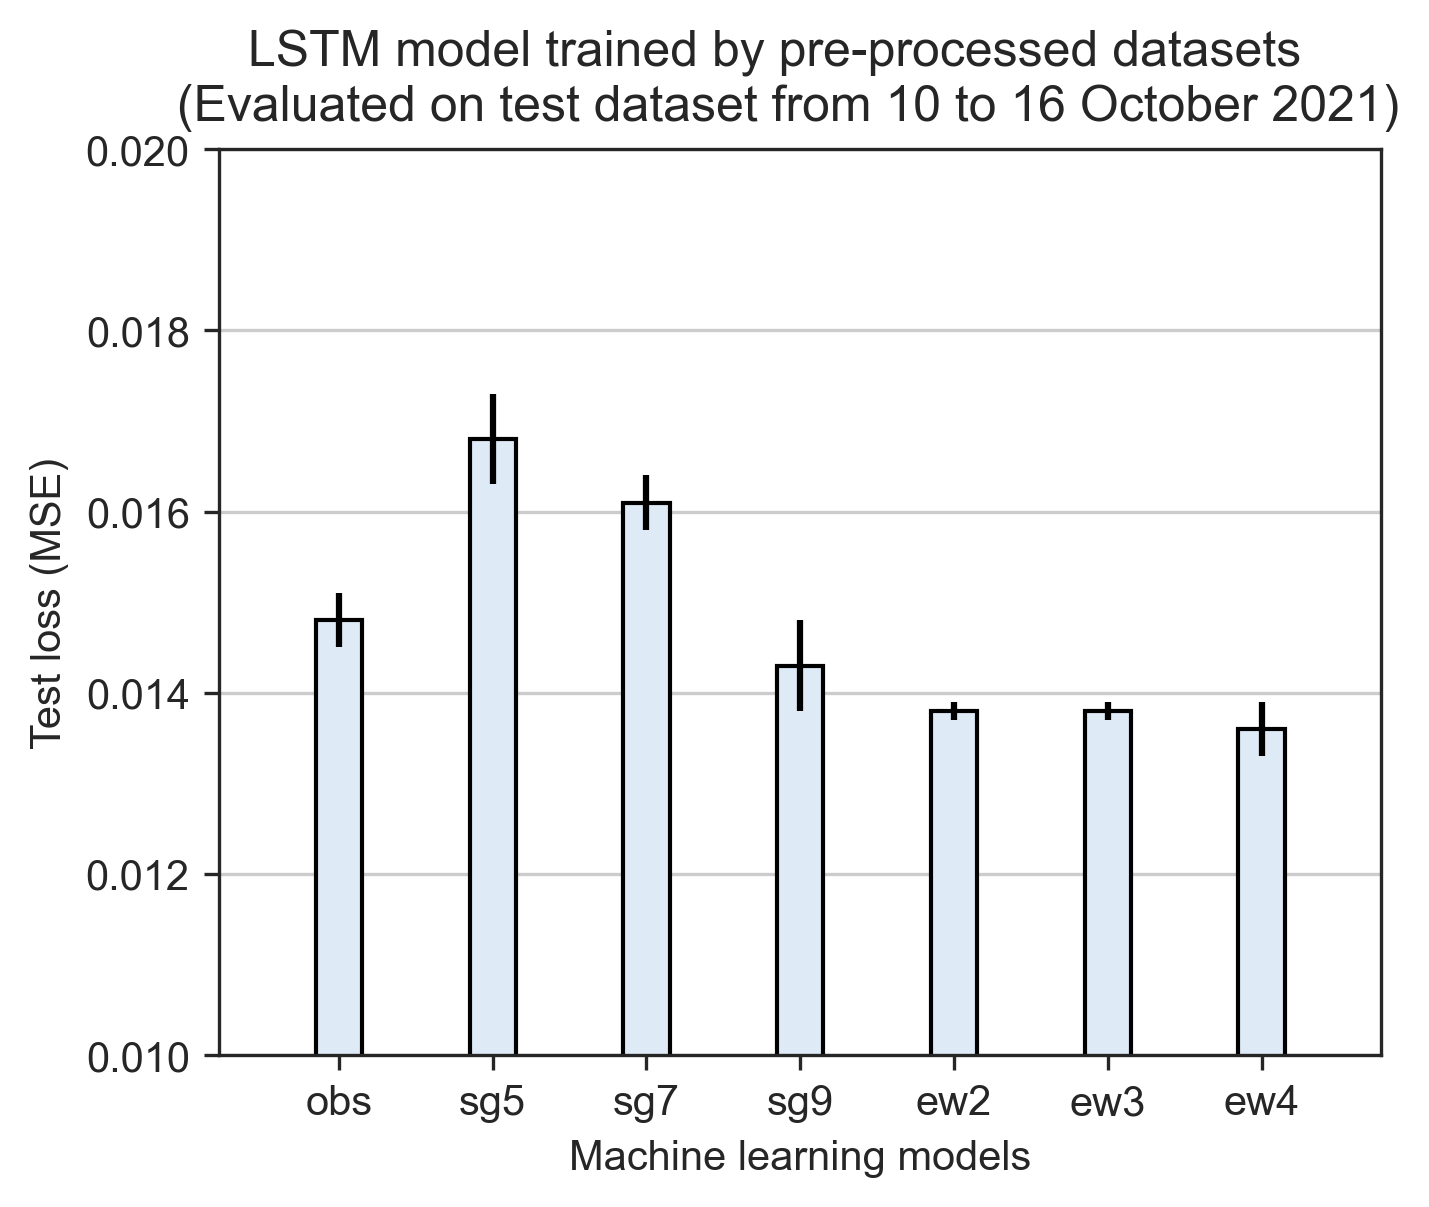
\includegraphics[width=\linewidth]{imgs/results/feature-engineering/pre-processing-colour.png}
    \caption{Baseline performance of colour forecasting models trained by LSTM.} \label{fig:preprocessing-colour}
  \end{subfigure}
\caption{Baseline performance of ammonia and colour forecasting models.} \label{fig:preprocessing-comparison}
\end{figure}

The influences of window sizes in data smoothing process are investigated using LSTM models and illustrated in Fig.~\ref{fig:preprocessing-comparison}. SG window sizes of higher and lower have different impacts on ammonia and colour forecasting models. For instance, LSTM-sg5 performed better than LSTM-sg9 in forecasting ammonia, LSTM-sg9 outperformed LSTM-sg5 in forecasting colour. The similar pattern can be observed in models trained by EWMA filters as well For ammonia forecasting model, LSTM-ew3 is better, while for colour forecasting model, LSTM-ew3 is better. Therefore, the window sizes of the data smoothing filters needs to be carefully selected. The unpredictable influences of applying data smoothing filters on forecasting models impedes the determination of the optimal data smoothing method in the subsequent experiments. For the futher studies, all the pre-processing methods will be applied on the LSTM models.

\section{Exploit hidden patterns in MBR effluent water quality to enhance model performance}
\subsection{Ammonia forecasting models}
In the section of feature engineering, we have introduced the selection and creation of the extra input features for training forecasting models as shown in Fig.~\ref{fig:feature-selection}. In this study, a forecasting model trained by 1 input is called an univariate model and denoted as LSTM-1; a forecasting model trained by 2 inputs is called a multivariate model and denoted as LSTM-2. For models trained by 3 and 4 inputs are denoted as LSTM-3 and LSTM-4. In Fig.~\ref{fig:nh3-feature-engineering}, the performance of ammonia forecasting models trained by 2 to 4 inputs (i.e., LSTM-2, LSTM-3, LSTM-4) are compared with the baseline performance (i.e., LSTM-1-obs) to demonstrate how the feature engineered features influenced on the model outputs. 
%Notice that due to colour data are not available from 10 to 16 October 2021, the models in Fig.~\ref{fig:colour-feature-engineering} were evaluated on training dataset from 16 to 22 January 2022. 

Leaving out the potential influences of heterogeneity between training and testing datasets on comparing the model performance, interesting resutls were still observed. As shown in Fig.~\ref{fig:nh3-feature-engineering}, LSTM-4-obs showed the highest test loss, followed by LSTM-3-obs, LSTM-2-obs and LSTM-1-obs. This result indicate that for LSTM models trained with more input featues can result in a poorer model performance. Based on our understandings to the extra features such as color levels and sine/cosine features, models trained with more inputs are expected lower test values. The model performance from LSTM-sg7 and LSTM-sg9 fits well with what we hypothesized. The results showed the test loss values of the LSTM models trained by datasets applied with sg7 and sg9 filters followed the trend of LSTM-4$<$LSTM-3$<$LSTM-2$<$LSTM-1. The most remarkable results are from LSTM models trained by datasets applied with SG filters at window size of 7. Comparing to the baseline model performance (i.e., LSTM-1-obs), the test loss values of LSTM-1-sg7, LSTM-2-sg7, LSTM-3-sg7 and LSTM-4-sg7 reduced by 4.2\%, 6.4\%, 7.9\%, and 8.9\%, respectively. 

Our findings in the results of ammonia forecasting models suggests that colour level is an indispensible input for improving the model performance. LSTM-2 models trained by datasets applied with any pre-processing methods showed lower test loss compared to LSTM-1, except LSTM-2 trained by dataset without applying any methods. There is a strong probability leads us to believe that the flucturation of ammonia concentration is highly correlated with the colour level in SHWEPP influent even without the direct evidence.

The methods of training LSTM models on pre-processed datasets have proved it's benefits in improving baseline model performance, yet the test loss values were only reduced slightly for those models trained with EWMA filtered datasets. As shown in Fig.~\ref{fig:nh3-feature-engineering}, LSTM-3-ew2, LSTM-4-ew2, LSTM-3-ew4 and LSTM-4-ew4 shared very similar test loss values to LSTM-1-obs, indicating the advantages of enhanced quality in training dataset were not fully reflected on the model performance when LSTM models were trained by EWMA filtered datasets.

\begin{figure}[h]
    \centering
    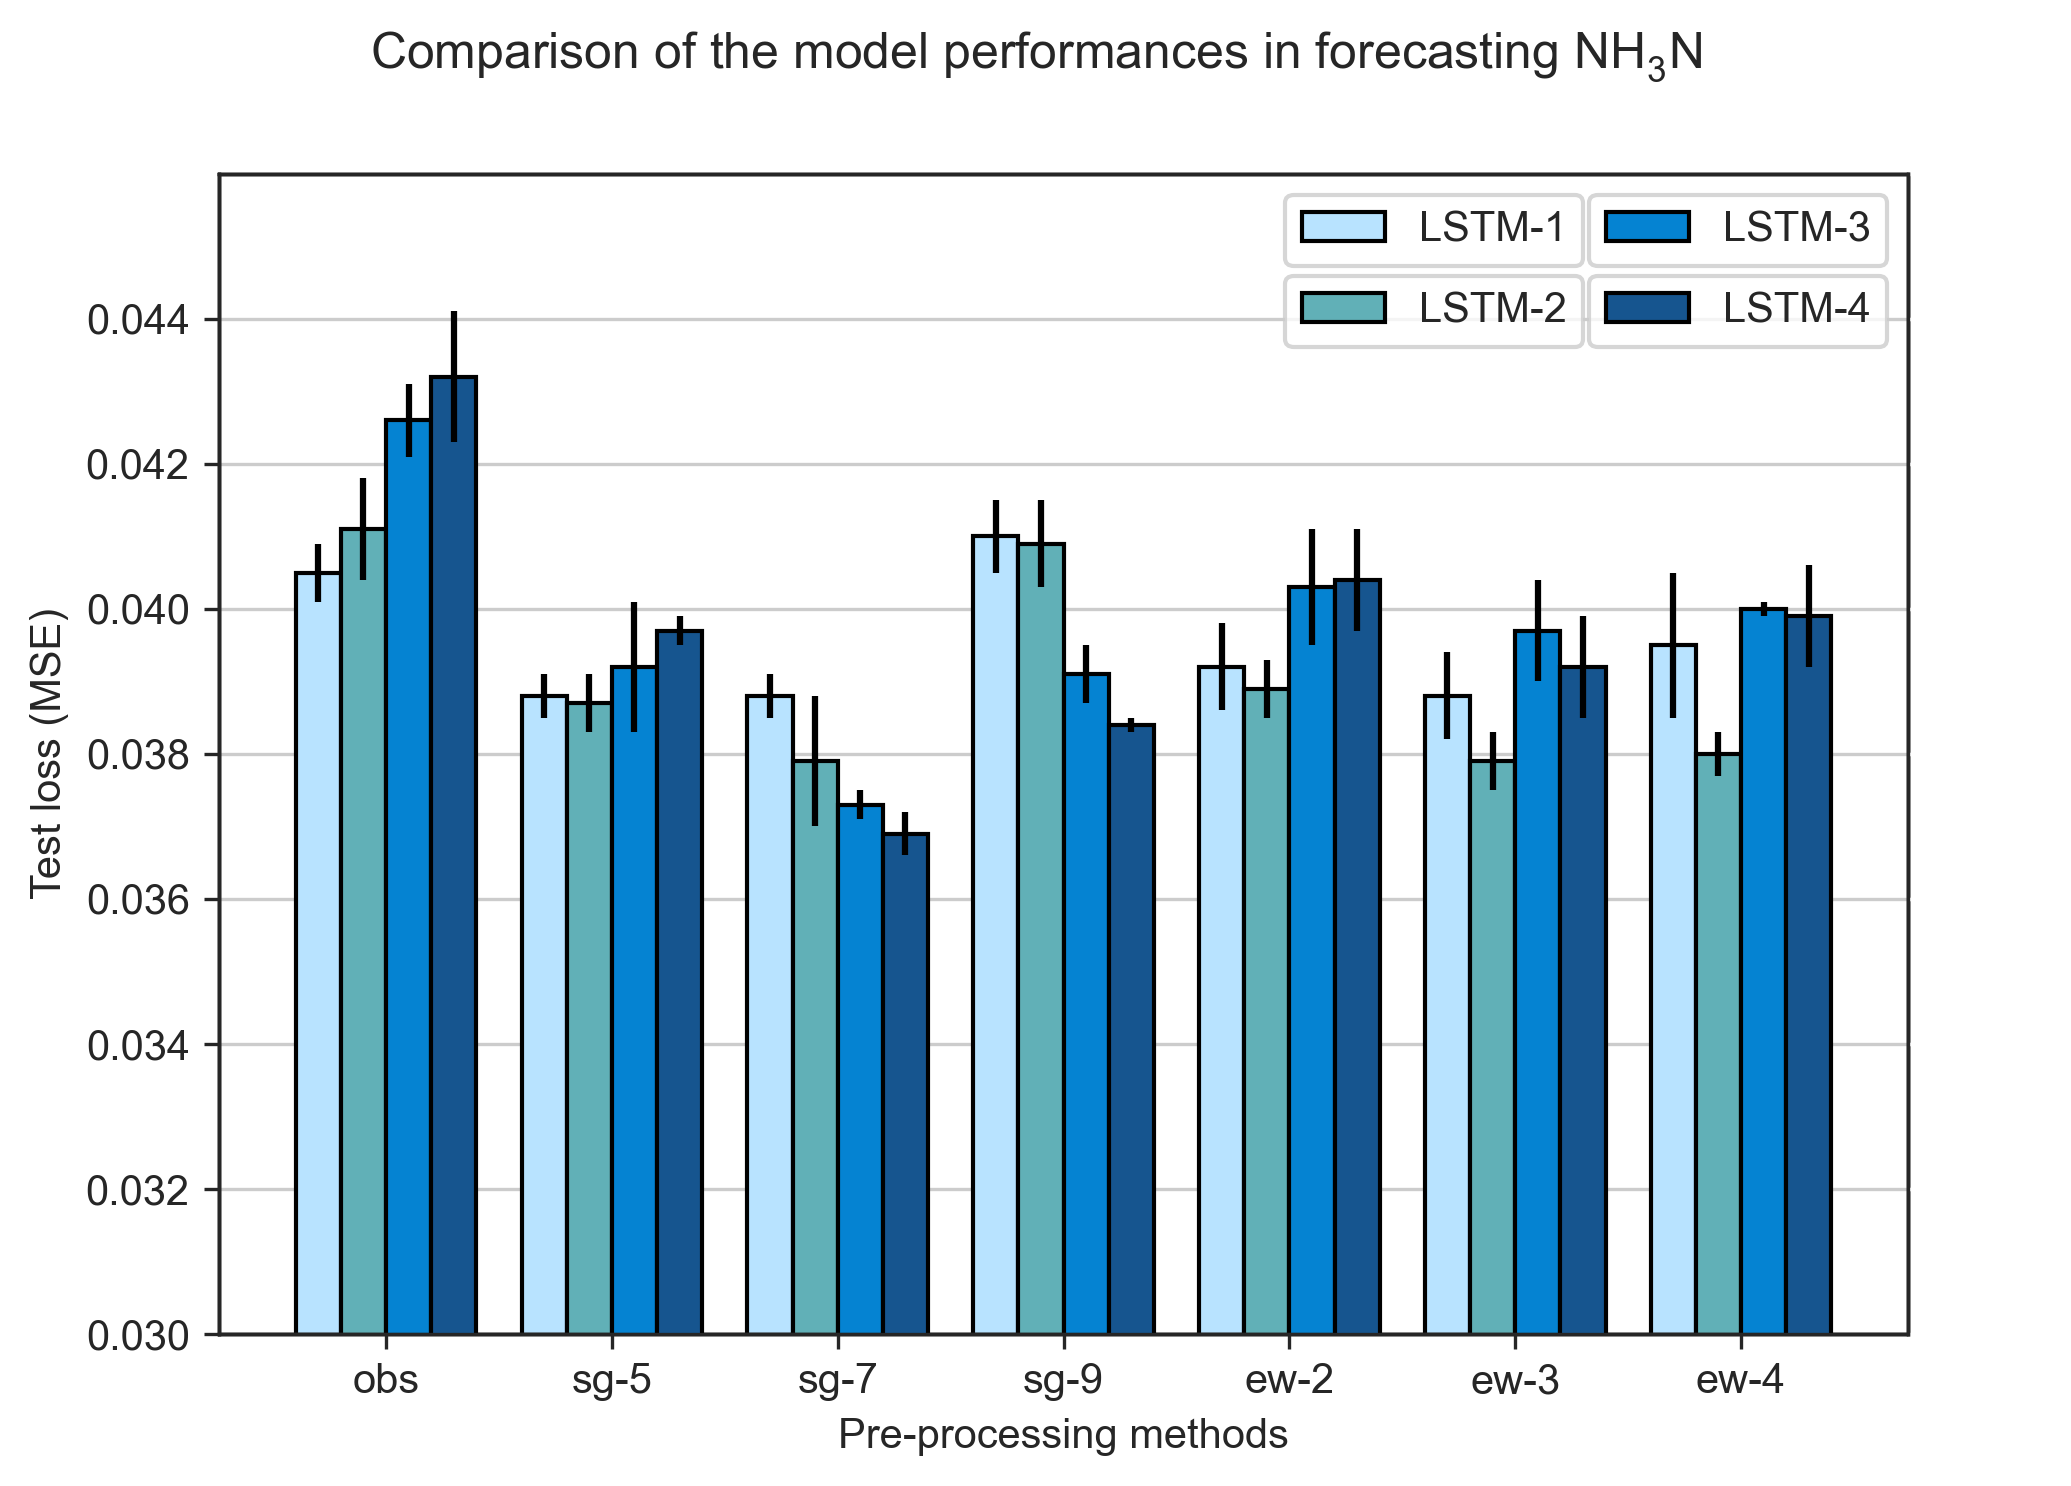
\includegraphics[width=0.6\columnwidth]{imgs/results/feature-engineering/nh3-input-1-4-comparison.png}
    \caption{Comparisons of the model performance in forecasitng ammonia concentrations.}
    \label{fig:nh3-feature-engineering}
 \end{figure}

\subsection{Colour forecasting models}

As shown in Fig.~\ref{fig:colour-feature-engineering}, most of the proposed pre-processing methods improved the performance of colour forecasting models. All the LSTM models trained by EWMA filtered datasets have lower test loss compared to the baseline model performance, while part of the LSTM models trained by SG filtered datasets showed improvement on the model performance. The performance of models trained by SG filtered datasets was rather disappointing. We observed that the test loss of LSTM-sg5, LSTM-sg7 and LSTM-sg9 showed much higher values of standard deviations, and this was probably as a result of the poor quality of the raw colour data. 

From the results of ammonia forecasting models, we thought that LSTM models trained by datasets applied with sg7 will generate the lowest test loss in LSTM-4, however, the results in the colour forecasting models revealed that the lowest test loss was generated from LSTM-3-sg9, with test values of 0.0121, a 28.6\% improvement in model performance compared to the baseline model performance. Contrary to expectations, datasets trained by four inputs failed to generate the lowest test loss. The fact of having higher test loss in LSTM-4 compared to LSTM-3 is evident and can be found in Fig.~\ref{fig:colour-feature-engineering} except LSTM-4-sg7. It is very likely that including ammonia concentrations as an input features worsened the quality of the training dataset and resulted in a poorer performance for colour forecasing models.


%\noindent
%\begin{myenumerate}
%    \item In the results of LSTM-sg7, the test values decreased with the increased number of model inputs, which satified the hypothesis we claimed in previous section.
%    \item The test loss values of LSTM-2 in all the pre-processed datasets are lower than LSTM-1 except for LSTM-obs, LSTM-sg9 and LSTM-ew2.
%    \item In LSTM-obs, models trained with more inputs resulted in poorer model performance, except for LSTM-obs, LSTM-sg9 and LSTM-ew2.
%\end{myenumerate}


\begin{figure}[t]
    \centering
    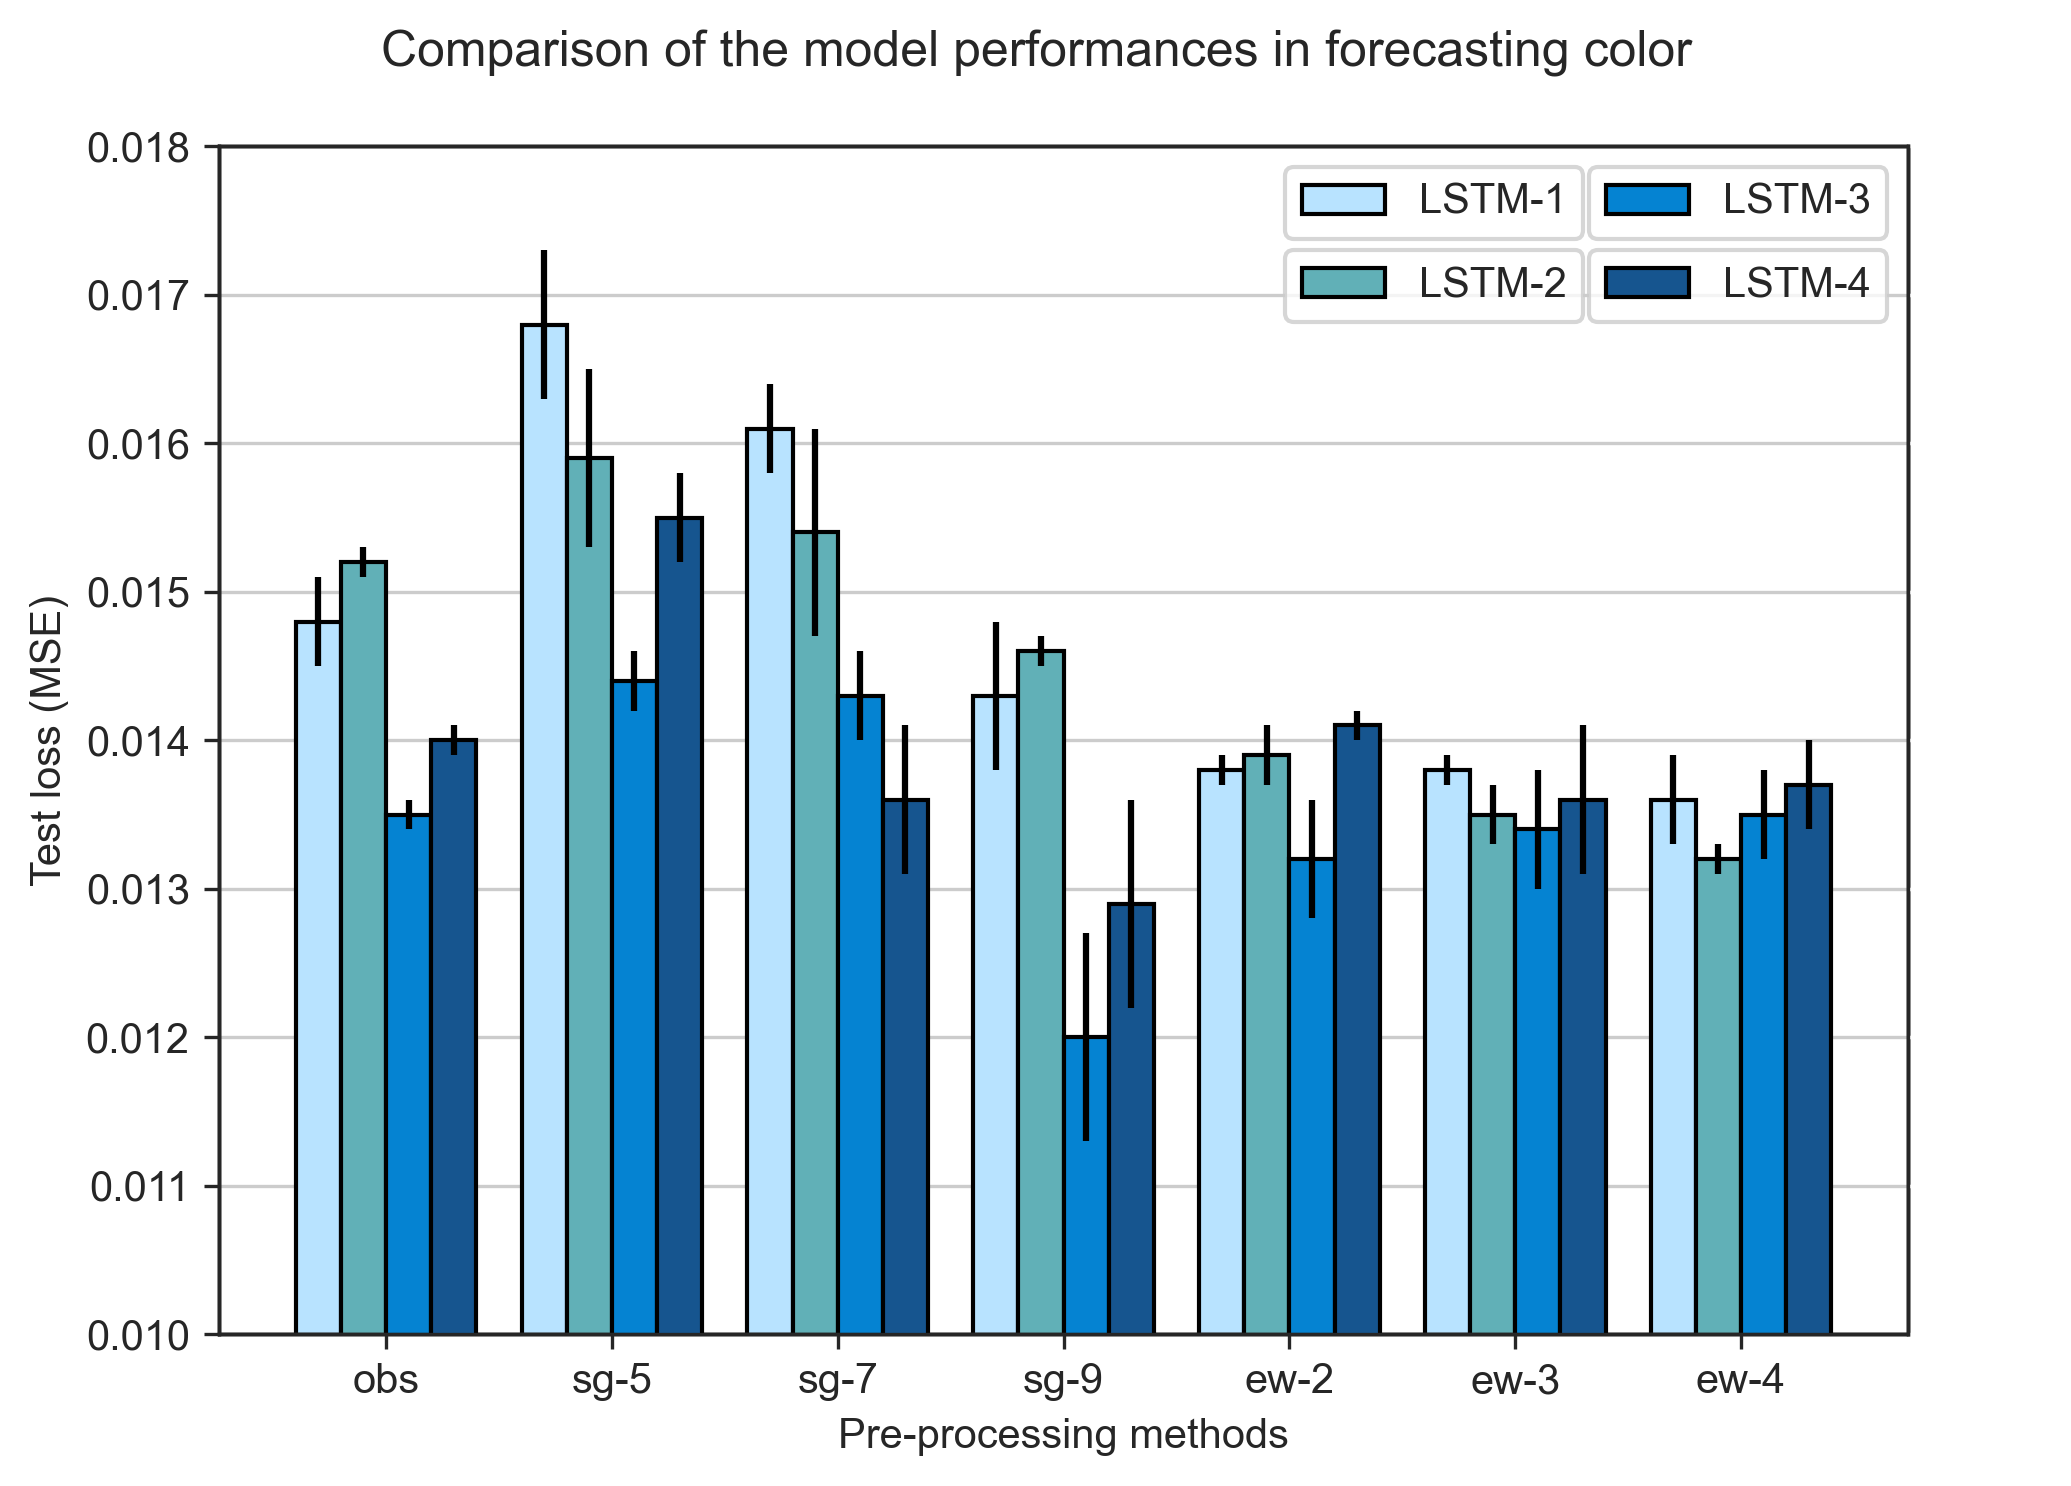
\includegraphics[width=0.6\columnwidth]{imgs/results/feature-engineering/colour-input-1-4-comparison.png}
    \caption{Comparisons of model performance in forecasting colour levels.}
    \label{fig:colour-feature-engineering}
 \end{figure}

%\section{Design of model architecture through analyzing wastewater composition in sewer system}
